\documentclass[conf]{new-aiaa}
%\documentclass[journal]{new-aiaa} for journal papers
\usepackage[utf8]{inputenc}

\usepackage{graphicx}
\usepackage{amsmath}
\usepackage{commath}
\usepackage[version=4]{mhchem}
\usepackage{siunitx}
\usepackage{longtable,tabularx}
\usepackage{float}
\usepackage{listings}
\usepackage{pdfpages}
\usepackage{color} %red, green, blue, yellow, cyan, magenta, black, white
\definecolor{mygreen}{RGB}{28,172,0} % color values Red, Green, Blue
\definecolor{mylilas}{RGB}{170,55,241}
\setlength\LTleft{0pt} 

\lstset{language=Matlab,%
	basicstyle=\footnotesize,
	breaklines=true,%
	morekeywords={matlab2tikz},
	keywordstyle=\color{blue},%
	morekeywords=[2]{1}, keywordstyle=[2]{\color{black}},
	identifierstyle=\color{black},%
	stringstyle=\color{mylilas},
	commentstyle=\color{mygreen},%
	showstringspaces=false,%without this there will be a symbol in the places where there is a space
	numbers=left,%
	numberstyle={\tiny \color{black}},% size of the numbers
	numbersep=9pt, % this defines how far the numbers are from the text
	emph=[1]{for,end,break},emphstyle=[1]\color{red}, %some words to emphasise
	%emph=[2]{word1,word2}, emphstyle=[2]{style},    
}

% ================================================================ % 
\title{ASE 389P.4 Methods of Orbit Determination \\ Homework 4: Reference Frames Transformations}

\author{Junette Hsin}
\affil{Masters Student, Aerospace Engineering and Engineering Mechanics, University of Texas, Austin, TX 78712}

\begin{document}

\maketitle

\begin{abstract}
	The transformation between an Earth	Centered Earth Fixed Earth frame and an Earth Centered Inertial frame is investigated. 


\end{abstract}


% ================================================================ % 
\section*{Problem}

 % \subsubsection*{Statement} 
\begin{center}
\fbox{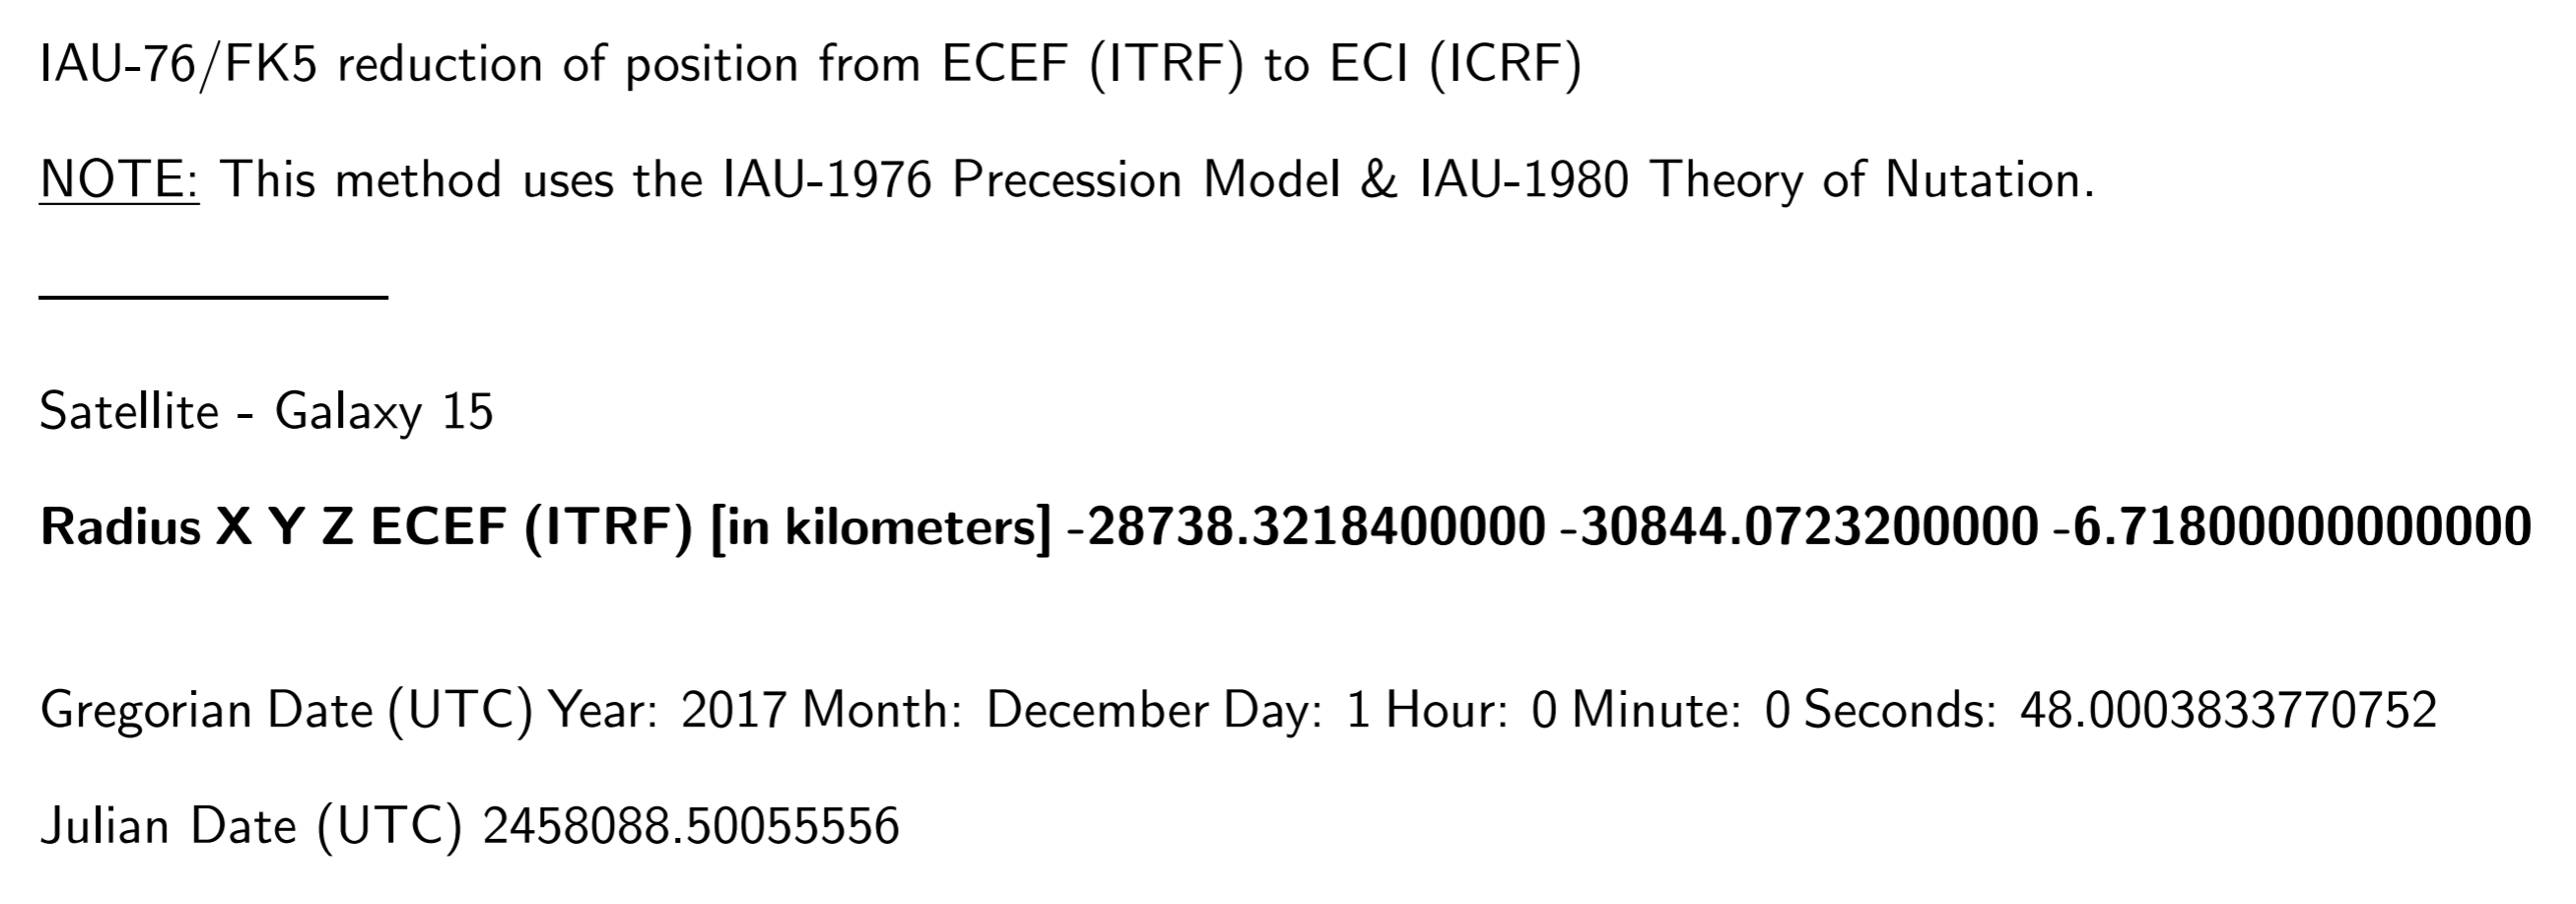
\includegraphics[width=0.9\textwidth]{prob_1.png}} \\
\end{center}

% ---------------------------------------------------------------- % 
\subsubsection*{Solution} 



\newpage
% ================================================================ % 
\section*{Appendix} 

\subsection*{HW4 MATLAB code} 

\begin{lstlisting}[basicstyle=\footnotesize]
% ASE 389 Orbit Determination
% HW 4
% Junette Hsin 

\end{lstlisting}

% ================================================================ % 

s\bibliography{sample}

\end{document}
